% -*- latex -*-
%%%%%%%%%%%%%%%%%%%%%%%%%%%%%%%%%%%%%%%%%%%%%%%%%%%%%%%%%%%%%%%%
%%%%%%%%%%%%%%%%%%%%%%%%%%%%%%%%%%%%%%%%%%%%%%%%%%%%%%%%%%%%%%%%
%%%%
%%%% This text file is part of the source of 
%%%% `Introduction to High-Performance Scientific Computing'
%%%% by Victor Eijkhout, copyright 2012-2022
%%%%
%%%% This book is distributed under a Creative Commons Attribution 3.0
%%%% Unported (CC BY 3.0) license and made possible by funding from
%%%% The Saylor Foundation \url{http://www.saylor.org}.
%%%%
%%%% array.tex : about array handling in programming languages
%%%%
%%%% THIS FILE IS NO LONGER USED
%%%%
%%%%%%%%%%%%%%%%%%%%%%%%%%%%%%%%%%%%%%%%%%%%%%%%%%%%%%%%%%%%%%%%
%%%%%%%%%%%%%%%%%%%%%%%%%%%%%%%%%%%%%%%%%%%%%%%%%%%%%%%%%%%%%%%%

\Level 0 {C arrays}
\lstset{language=C}

\Level 1 {Static arrays}
\label{sec:c-array-static}

The easiest way to create arrays is with the `square bracket notation':
\begin{lstlisting}
int x[5];
int y[6][7];
\end{lstlisting}

The same square brackets are used for indexing:
\begin{lstlisting}
for (int row=0; row<nrows; row++)
  for (int col=0; col<ncols; col++)
    moments[row][col] = pow( coefficient[row],(double)col );
\end{lstlisting}

In these examples we used a constant for the array bound.
See section~\ref{sec:c-vla} for using a variable.

\Level 2 {Allocation}

What we are calling `static' arrays are actually technically called
\indextermsub{automatic}{array}s.
Static arrays are arrays with the keyword \indextermtt{static}:
\begin{lstlisting}
static float x[5]; // a truly `static' array
int main() {
  float y[6]; // this one is `automatic'
}
\end{lstlisting}

Automatic arrays, which we will from now on call `static',
are usually allocated on the
\emph{stack}\index{stack!array creation on},
because they have static scope:
\begin{lstlisting}
// variables `x' and `y' don't exist
if (whatever) {
  int x;
  float y[2];
  // variables `x' and `y' exist for the duration of the conditional
  ....
}
// variables `x' and `y' don't exist anymore
\end{lstlisting}
Thus, creating too many of these may lead to \indextermbus{stack}{overflow}.
Check out the \indextermunix{limit} command.

\Level 2 {Passing to functions}

You can pass an array to a function,
indicating in the function prototype that it is an array.
However, the function can not query the array length,
so that has to be passed separately if this information is needed.

\snippetwithoutput{cansiset1d}{code/array}{set1d}

You can also use the equivalence of arrays and pointers:

\snippetwithoutput{cansisetstar}{code/array}{setstar}

\Level 1 {Multi-dimensional arrays}

Declaring a multi-dimensional array:
\begin{lstlisting}
int y[6][7];
\end{lstlisting}

Initialization:
\begin{lstlisting}
int z[2][2] = { {1,2},{3,4} };
\end{lstlisting}

Such arrays are stored in \indexterm{row-major} ordering,
meaning that rows are contiguous in memory.

\snippetwithoutput{cansiset2d}{code/array}{set2d}

Passing them to functions is a little more tricky:
all dimensions except the first have to be pass explicitly.

\snippetwithoutput{cansiset2d}{code/array}{pass2d}

\Level 1 {Variable-length arrays}
\label{sec:c-vla}

In \indextermsub{Ansi}{C}, arrays had to be declared with compile-time bounds,
as above.
The \emph{C99}\index{C!99} standard has added \indextermsub{variable-length}{array}s:

\snippetwithoutput{c99array}{code/array}{set99}

\begin{itemize}
\item These arrays are still `automatic' so they only live in the
  scope where they are defined.
\item The term `variable-length' does not mean that the length
  is variable; only that it is specified with a variable.
  Resizable arrays only exist in~C++; see section~\ref{sec:cpp-std-vector}.)
\item 
  Such declarations can also be done in multi-D.
  However, they are pointless for passing arrays to functions.
\item 
  Note: this mechanism was already available as an extension
  on many compilers before the C99 standard.
\end{itemize}

\Level 1 {Dynamically allocated arrays}

Before C99's variable-length arrays,
the only way to create arrays with a size determined at run-time
was through \indextermsub{dynamic}{allocation},
using the \indextermtt{malloc} keyword. This
\begin{enumerate}
\item takes an argument that is a number of bytes, and
\item returns the address of a block of memory of that size.
\item It returns zero if the block could not be created.
\end{enumerate}
\begin{lstlisting}
int arraysize = 500;
float *x;
x = (float*) malloc( arraysize*sizeof(float) );
if (!x) printf("Could not allocate x\n");
\end{lstlisting}

Indexing, both in the scope where the array is created,
and in subprograms it is passed to,
is exactly the same as above.
For passing such arrays to functions, the type is now \lstinline+float*+:
%
\snippetwithoutput{cmallocpass}{code/array}{cmalloc}

\Level 1 {Dynamic arrays, scope, memory leaks}

The memory allocated for dynamic arrays is not subject to scope:
\begin{lstlisting}
void create( float **x,int len ) {
  float *x_space = (float*) malloc(len*sizeof(float));
  *x = s_space;
}
int main() {
  float *x;
  create(&x,50);
}
\end{lstlisting}
Thus, this allocation has to happen on the
\emph{heap}\index{head!array creation on}
This is good for flexible programming, but
may lead to \indexterm{memory leak}s.

\Level 1 {Multi-dimensional dynamic arrays}

Solution 1:
\cverbatimsnippet{cmallocsizenn}

This allocates a single block,
consisting of arrays of length~\n{cols}:
\snippetwithoutput{cmallocsizenn3}{code/array}{rowlength}

Solution 2:\\
create a one-dimensional array,
and convert multi-dimensional indices to one-dimensional.

\snippetwithoutput{cmalloc2d}{code/array}{cmallocpass}

\Level 1 {Type theory of arrays}

After declaring
\begin{lstlisting}
int x[5][6];
\end{lstlisting}
the expression \lstinline{x[3]} stands for an array of length~6,
compatible with being an \lstinline+int*+.

Does that mean that \lstinline{x} itself is of type \lstinline+int**+?
No, it is not.
Careful parsing of the standard shows that \lstinline{x} itself
is also of type \lstinline+int*+!
Above you already saw that multi-dimensional arrays are contiguous in memory,
so you can step through their content with pointer arithmetic.

Let's explore the notion of \lstinline+int**+ and arrays a little more.
You can in fact write:
\begin{lstlisting}
int **x;
x = (int**)malloc( nrows*sizeof(int*) );
for (int irow=0; irow<nrows; irow++)
  x[irow] = (int*)malloc( ncolumns*sizeof(int) );
\end{lstlisting}
and the resulting object can also be indexed with~\lstinline+x[i][j]+.
However, this has significant disadvantages:
\begin{enumerate}
\item The `array' is no longer contiguous, so you can not easily step through the contents.
\item Copying its contents is harder than copying contiguous data.
\item The performance of operations may suffer because of the lack of locality and regularity.
\end{enumerate}

\Level 0 {C++ arrays}

The C arrays described above are available in C++,
with exception of variable-length arrays.
However, better mechanisms exist.

\Level 1 {Array}

\lstset{language=C++}

The C++ \lstinline+std::array+ is close to the C `static arrays'
(section~\ref{sec:c-array-static})
in that it requires bounds that are known at compile time.
\begin{lstlisting}
std::array<float,8> eight_floats;
\end{lstlisting}
Note that the size is a template parameter, not a parameter of the constructor.

While the compile-time bound is a severe restriction on flexibility,
this is the most efficient array variant in C++:
\begin{itemize}
\item There is no storage overhead in addition to the element storage;
\item Nested arrays of this type are form contiguous memory;
\item The compiler can optimize these arrays as much as the C-style static arrays.
\end{itemize}
However, storage for these arrays happens on the heap,
rather than on the stack as for C static arrays.

The convenience of having methods such as \lstinline{size}
and bound checking through \lstinline{at}
makes these arrays preferable over the C variant.

\Level 1 {Vector}
\label{sec:cpp-std-vector}

The \lstinline+std::vector+ also creates space on the heap.
By contrast with \lstinline+std::array+
\begin{itemize}
\item the size can be specified as a dynamically determined quantity; and
\item the size can be changed.
\end{itemize}
This first difference means that the vector now needs a control block that
contains the size and the allocated capacity.
The second difference implies that certain operations can be
computationally inefficient.

\Level 0 {Fortran}

\Level 1 {Static}

\lstset{language=Fortran}

Arrays can be created with compile-time bounds:
\begin{lstlisting}
Integer,dimension(5) :: x
Integer,parameter :: size = 6
Integer,dimension(size,size) :: y
\end{lstlisting}

These arrays are scoped.

Unlike in C, Fortran arrays can have a specified lower bound:
\begin{lstlisting}
Integer,dimension(-1:7) :: x
\end{lstlisting}

\Level 1 {Dynamic}

\begin{lstlisting}
Real*4,dimension(:),allocatable :: x
Integer :: n

Read *,n
Allocate(x(n))
\end{lstlisting}

Such arrays are also scoped,
and can therefore not lead to memory leaks,
unlike \lstinline{malloc}'ed arrays in~C.

\Level 1 {Memory layout}

Fortran arrays are column-major:
the columns are stored contiguously.
For higher dimensions this is also phrased as
`the first index varies quickest'.

\Level 0 {Layout in memory}
\label{sec:CFarrays}
\index{C!array layout|(}
\index{Fortran!array layout|(}

C and Fortran have different conventions for storing multi-dimensional
arrays. You need to be aware of this when you pass an array between
routines written in different languages. 

Fortran stores multi-dimensional arrays in \indexterm{column-major}
order; see figure~\ref{fig:cf-arrays}.
For two dimensional arrays \texttt{A(i,j)} this means that
the elements in each column are stored contiguously: a $2\times2$
array is stored as \texttt{A(1,1), A(2,1), A(1,2), A(2,2)}. Three and
\begin{figure}[ht]
  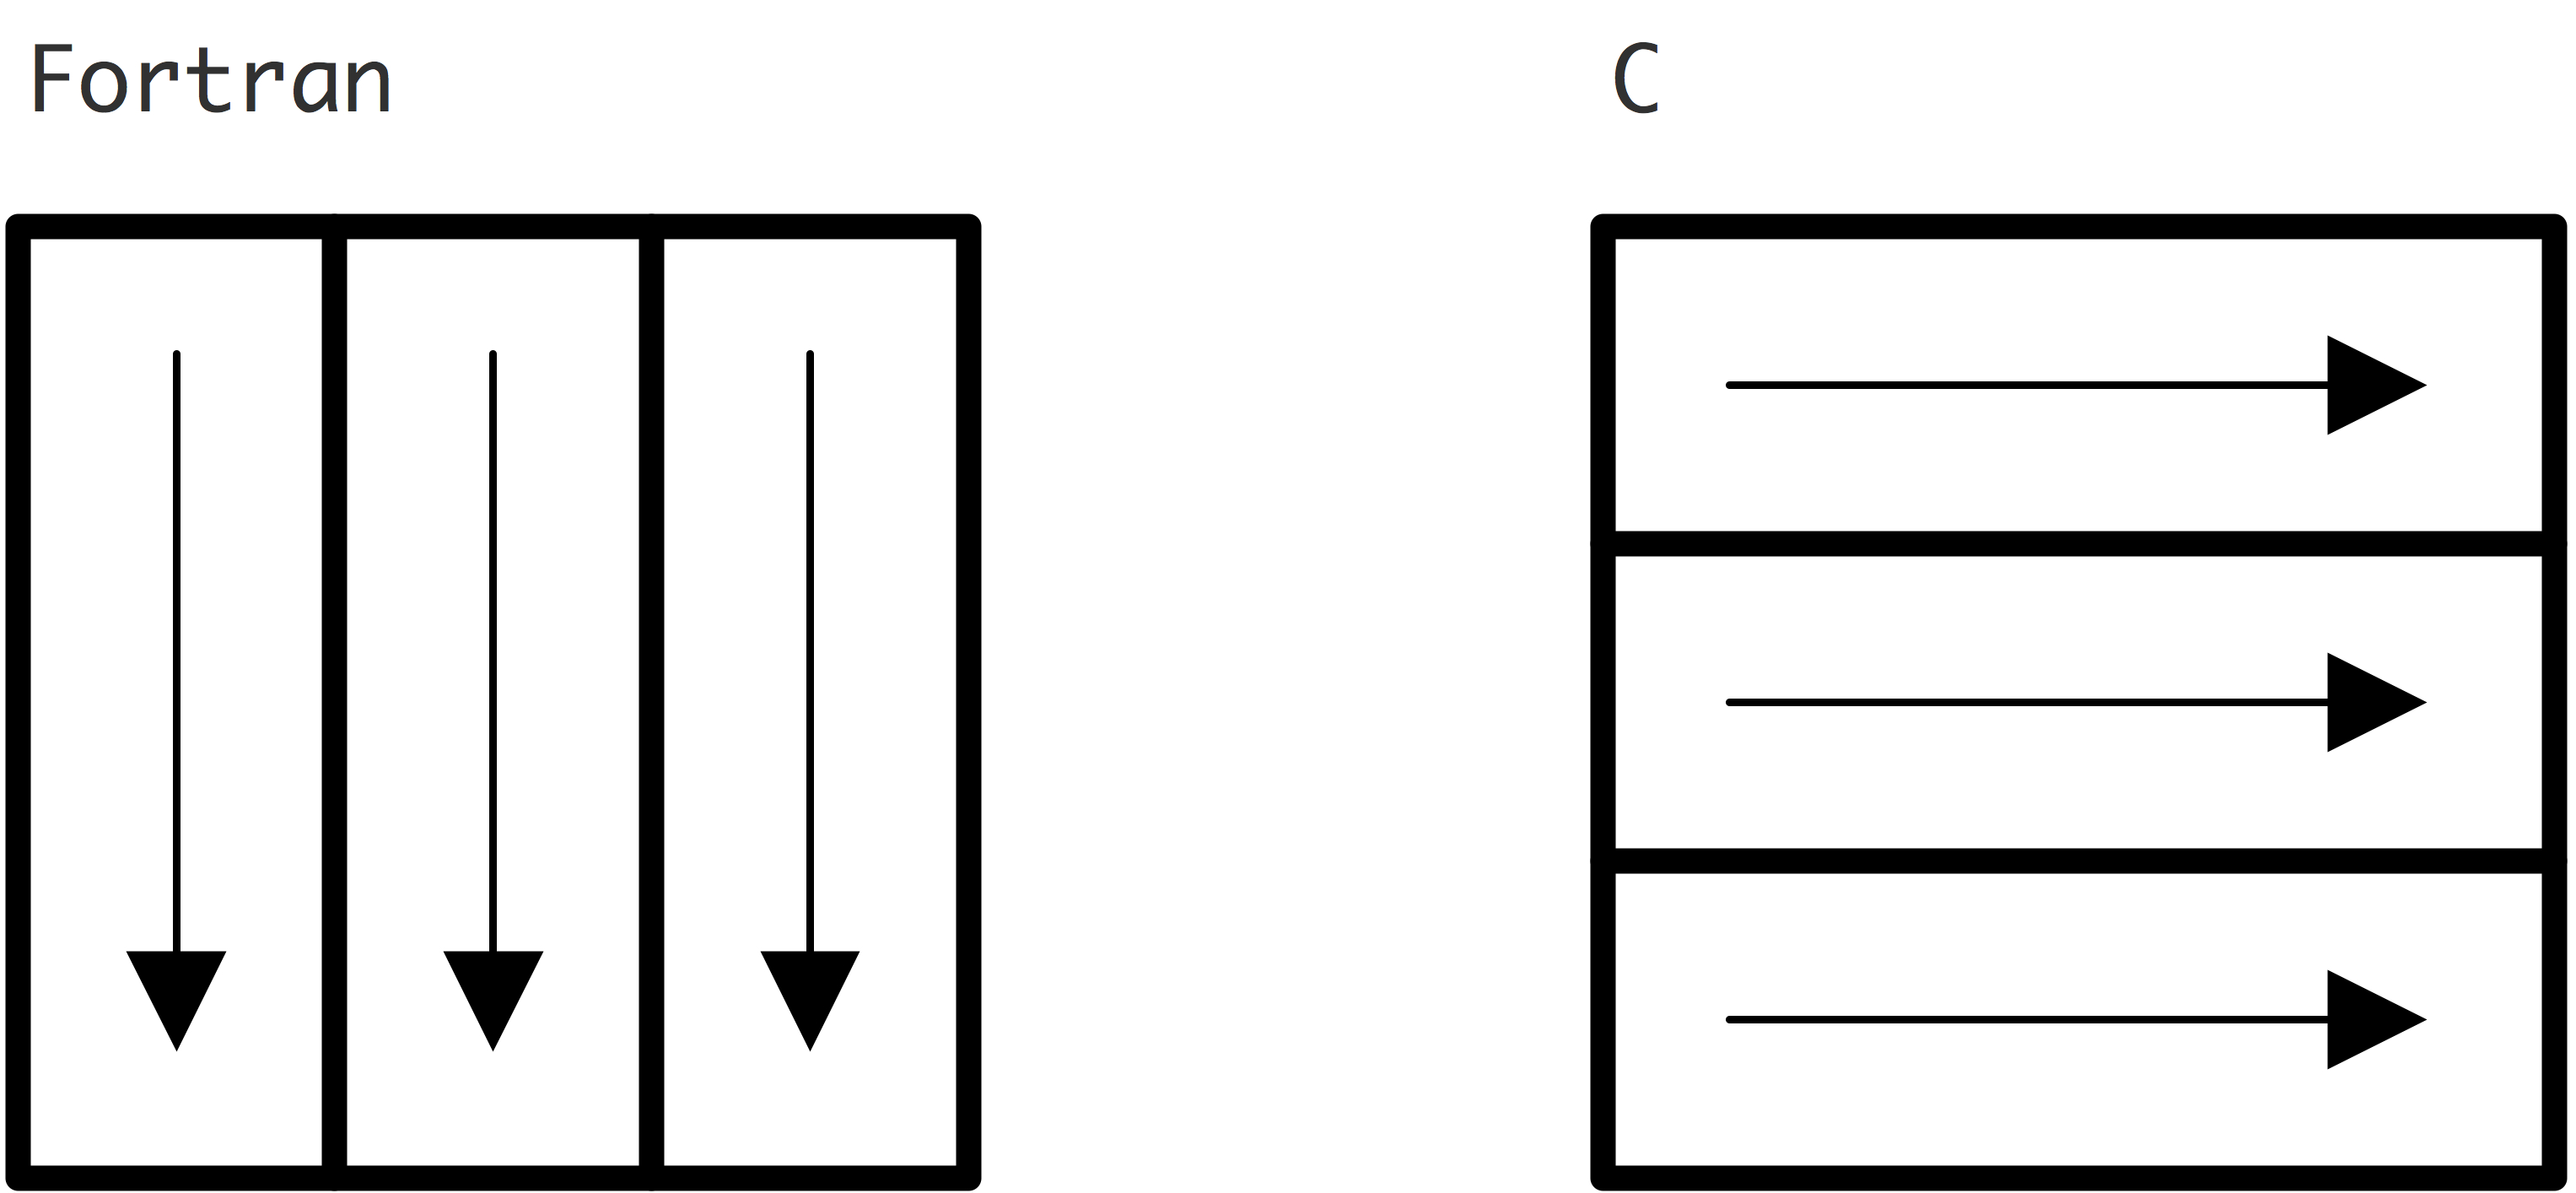
\includegraphics[scale=.13]{cf-arrays}
  \caption{Fortran and C array storage by columns and rows respectively.}
  \label{fig:cf-arrays}
\end{figure}
higher dimensional arrays are an obvious extension: it is sometimes
said that `the left index varies quickest'.

C arrays are stored in \indexterm{row-major} order: elements in each
row are stored contiguous, and columns are then placed sequentially in
memory. A~$2\times2$ array \texttt{A[2][2]} is stored as
\texttt{A[1][1], A[1][2], A[2][1], A[2][2]}. 

A number of remarks about arrays in~C.
\begin{itemize}
\item C (before the C99 standard) has multi-dimensional arrays only in
  a limited sense. You can declare them, but if you pass them to another
  C function, they no longer look multi-dimensional: they have become
  plain \texttt{float*} (or whatever type) arrays. That brings us to
  the next point.
\item Multi-dimensional arrays in C look as if they have type
  \texttt{float**}, that is, an array of pointers that point to
  (separately allocated) arrays for the rows. While you could
  certainly implement this:
\begin{verbatim}
float **A;
A = (float**)malloc(m*sizeof(float*));
for (i=0; i<n; i++)
  A[i] = (float*)malloc(n*sizeof(float));
\end{verbatim}
  careful reading of the standard reveals that a multi-dimensional
  array is in fact a single block of memory, no further pointers
  involved.
\end{itemize}
Given the above limitation on passing multi-dimensional arrays, and
the fact that a C~routine can not tell whether it's called from
Fortran or~C, it is best not to bother with multi-dimensional arrays
in C, and to emulate them:
\begin{verbatim}
float *A;
A = (float*)malloc(m*n*sizeof(float));
#define SUB(i,j,m,n) i+j*m
for (i=0; i<m; i++)
  for (j=0; j<n; j++)
    .... A[SUB(i,j,m,n)] ....
\end{verbatim}
where for interoperability we store the elements in column-major fashion.

\index{C!array layout|)}
\index{Fortran!array layout|)}

\Level 1 {Array alignment}
\index{cacheline!boundary alignment|seealso{allocation, aligned}}

For reasons such as \ac{SIMD} \indexterm{vector instructions}, it can
be advantageous to use \indextermsubdef{aligned}{allocation}. For
instance, `16-byte alignment' means that the starting address of your
array, expressed in bytes, is a multiple of~16.

In~C, you can force such alignment with 
\indextermtt{posix_memalign}. In Fortran there is no general
mechanism for this. The Intel compiler allows you to write:
\begin{verbatim}
double precision, allocatable :: A(:), B(:)
!DIR$ ATTRIBUTES ALIGN : 32 :: A, B
\end{verbatim}


% LocalWords:  Eijkhout
